\documentclass[a4paper]{scrartcl}

\usepackage[comma, sort&compress]{natbib}
\usepackage[english]{babel}
\usepackage{microtype, amsmath, setspace, marvosym, graphicx}
\doublespacing

%opening
\title{Valuing Road-Transport Noise Abatement Measures}
\author{Duco de Vos}

\begin{document}
	
\maketitle
	
\section{Introduction}
	
Transport noise is a costly affair. Substantial noise-levels can cause annoyance, stress and illness.   According to a European report \citep{CEDelft2011}, the external cost of noise induced by road transport in Europe\footnote{EU27 excluding Malta and Cyprus, including Norway and Switzerland.} amounts to \EUR17 Billion annually. In Europe the Environmental Noise Directive \footnote{European Commission, 2002. Environmental noise directive 2002/49/EG.} aims to reduce harmful noise-exposure of citizens. Without specifying limit noise-values, this directive still gives governments the incentive to devise policy-measures against noise. The main goal of noise-abatement policy measures is to minimize the external costs of noise, arising in the absence of a market for tranquillity \citep{Nelson2008}. In the Netherlands these external costs may, partly, be mitigated by road- and fuel taxes \citep{Andersson2013}, in combination with policy measures such as silent tires, silent tarmac, traffic management systems (TMS), highway sound-barriers and housing-insulation \citep{RIVM2001}.
	
Within this maze of policy-measures and different taxes, it seems difficult to evaluate the current situation in the Netherlands against the socially optimal outcome, where the marginal costs of abatement (e.g. construction costs of sound barriers, implementation costs of TMS etc.) equal the marginal benefit of abatement (i.e. marginal willingness-to-pay for noise reduction). The objective of this paper is to develop a framework from which the economic efficiency of transport-noise policy measures can be evaluated. Although several meta-analyses on this subject exist (most notably \cite{Nelson2008}), the relevance of the current paper lies in the focus on the Netherlands, the explicit connection made with cost-benefit analysis (CBA), and the in-depth exploration of (novel) stated preference methods. Section 2 gives an overview of the current academic debate concerning noise-abatement policy, section 3 elaborates on strategies to estimate the willingness-to-pay for noise reduction, section 4 proposes a research framework based on the discussion in the preceding sections and section 5 concludes.
	
\section{Noise-abatement policy}

Since the 1920s, the first-best solution to external costs in motoring is generally regarded to be a ``road-pricing" scheme that charges drivers the marginal external costs they impose on others (in terms of congestion, environmental damage, noise etc.) \citep{Pigou1924}. Electronic Road Pricing (ERP) schemes can nowadays be used to charge motorists a regulatory fee that can be differentiated along many dimensions (trip length, vehicle type etc.) in order to reflect the appropriate marginal external costs imposed \citep{Verhoef1995}. Although ERP schemes are technically feasible, social and political issues prevent such systems from being introduced widely. When road-users are not taxed for the negative effects of the noise they produce, this noise will be overproduced. Still, an array of policy tools is developed to tackle the problem of traffic noise.
	
\begin{figure}[h]
	\caption{Factors causing adverse noise-effects, based on \cite{Nijland2003}}
	\centering
	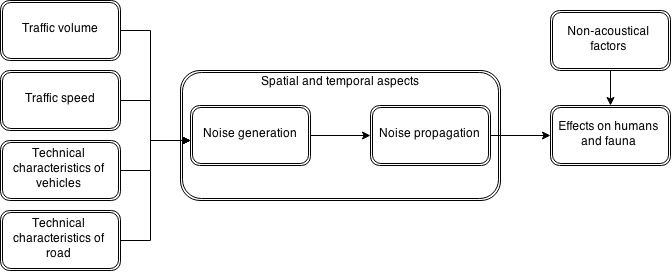
\includegraphics[width=0.8\textwidth]{Graph0}
\end{figure}
	
The amount of  noise that an individual vehicle produces depends on the vehicles technical construction (type of motor, tires etc.), driver characteristics (driving speed and style), and on the type of road surface (see Figure 1). Source-based policy measures are designed to limit noise generation: restrictions on motor and tire noise are placed at the EU level\footnote{European Commission, 2007.  Vehicle type approval framework directive 2007/46/EC.}, decisions on road surfaces (such as the implementation of silent tarmac) are made at a more local level. Traffic volume, the amount of lorries, and traffic speed affect noise-levels greatly. Traffic-management systems influence the maximum speed and the flow of traffic and can therefore be used to limit noise-generation. Next to measures that limit noise-generation, the government can take steps in hampering noise propagation, through noise barrier walls and, ultimately through housing insulation.  Measures that tackle noise generation are generally considered to be more cost-effective than measures that hamper noise propagation \citep{DanishRoadInstituteDRI2005,DenBoer2007}.
	
An aspect of transport policy that is often overlooked in economics literature is the social and political acceptability of transport measures. A Swedish psychological study, using a questionnaire, done by \cite{Eriksson2008} emphasizes the importance of facilitating alternative modes of transport in combination with restrictive traffic management systems. Measures that restrict the amount of cars on the road are more likely to be accepted when alternative travel options are made more accessible. On the basis of another survey, \cite{Rienstra1999} point out that noise annoyance is not generally regarded as a social problem. This might influence the political feasibility of noise-abatement measures negatively. They argue that influencing problem perception, by better informing people, might be one of the most effective ways to increase social- and political acceptability for transport-policy measures.
	
In the study done by \cite{Nijland2003} different policy measures, such as silent tires and the implementation of silent tarmac, are evaluated on the noise-reduction (in dB(A)) they constitute, the unit costs involved and the total costs to society. These costs are derived from different expert reports regarding policy measures in the Netherlands. With respect to road-transport noise, costs of introducing mandatory silent tires and silent tarmac on all main roads are estimated, but would need to be reconsidered and estimated when conducting research today, due to changed conditions.  The exclusion of highway-noise barriers and housing insulation costs, and the use of very general values for willingness-to-pay (based on a several meta-analyses) pose some limitations to this study. However, the equal treatment of the costs and benefits involved in noise-abatement projects in this study is a valuable addition to the existing literature.

\section{Willingness-to-pay for noise reduction}

As external effects are not (correctly) priced in the market, valuing these effects poses a problem. Academic literature describes various solutions to the problem of estimating the value of external effects. Hedonic Pricing (HP) and Contingent Valuation (CV) methods are the most frequently used tools in uncovering the willingness-to-pay/accept (WTP/WTA) for external effects. Next to these widely used research tools some obscure methods, such as ``quality-of-life"-surveys are used as a means to the same end \citep{VanPraag2005}. This section describes in detail the workings and application of HP and CV methods, and briefly touches upon more innovative methods of WTP-estimation.

\subsection{Hedonic pricing methods}

Valuing external effects with the use of revealed preference methods is possible in the presence of private markets that are complementary to externality-avoidance, such as the market for housing \citep{Nelson2008}. Theoretically, a discount for noise can be obtained through analysing the market values of identical houses in an environment with, and an environment without noise. This implies that people with a lower willingness-to-pay for noise-avoidance will locate in noisy areas, and people with a high willingness-to-pay will locate in more quiet areas. The resulting equilibrium can be disturbed in case of (durable) shocks in noise-levels, in which case a new stable equilibrium will arise. In reality the characteristics-spectrum of a house is much more complex, and a noisy environment can be offset by other positive characteristics.

\cite{Rosen1974} defines hedonic prices as 
\begin{quote}``\dots implicit prices of attributes (\dots) revealed (\dots) from observed prices of differentiated products and the specific amounts of characteristics associated with them."\end{quote} 
This entails that, in hedonic pricing models, the willingness-to-pay for a product is subdivided in terms of product characteristics and attributes. The 4 main assumptions for the operation of hedonic pricing analysis are defined by \cite{Bateman1993}:
\begin{enumerate}
	\item Aggregate willingness-to-pay reflects the social benefit.
	\item Environmental quality changes are perceivable, and they affect the future benefits from owning a property, thus people are willing to pay for these quality changes.
	\item The area considered is a competitive market with free access and perfect information on prices and environmental quality.
	\item The housing market is in always equilibrium.
\end{enumerate}

An early hedonic pricing analysis of highway noise, done by \cite{Nelson1982} specifies a model:
\begin{equation}
V = V(Q, Z)
\end{equation}

In which $V$ represents a vector of housing price observations, $Q$ a vector of environmental quality characteristics, $Q_j$ the level of tranquillity, and $Z$ a vector of all other housing characteristics. $\frac{\partial V}{\partial Q_j }$ then represents the marginal price of tranquillity. Evaluating  $\frac{\partial V}{\partial Q_j }$ for different levels of $Q_j$ results in an estimated price function of noise/tranquillity. Noise sensitivity of housing prices is often evaluated by the Noise Depreciation Index (NDI) \citep{Walters1975}. For highway noise, \cite{Nelson1982} defines the NDI as the difference in total percentage depreciation divided by the difference in noise exposure, for residential properties that differ only in terms of noisy environment.	

Besides the obvious advantage of HP-studies that they are based on real-world choices, some drawbacks to this approach exist as well. Assumption 3 and 4 as defined above, for instance, are highly unlikely to be realistic: It is doubtful whether there is perfect information concerning housing prices and environmental quality among individuals, and the housing market seems plagued with market imperfections.

In the Dutch context, noise-valuation studies on the basis of HP are particularly scarce. A study by \cite{Theebe2004} estimates NDI values for the western part of the Netherlands, using a Spatial-error model in combination with HP. Spatial error models deal with spatially correlated standard errors in an Ordinary Least Squares estimation context. The spatial error model that \cite{Theebe2004} uses might be appropriate because residences located near each other might share neighbourhood and construction characteristics. The results of this paper indicate a NDI value between 0.3\% and 0.5\% per dB(A), above the 65 dB(A) threshold. This means that, on average, a house worth \EUR200.000 loses between 3\% and 5\% of its value (a \EUR6000-10000 decline) with a 10 dB(A) increase in noise-levels. 

Other “Spatial Econometrics” approaches towards HP include Spatial-lag models, that account for systematic spatial information that is not included in the variables of the OLS model. The paper by \cite{Pope2008} (elaborated on in the next paragraph) uses such a model. Besides correction for systematic spatial disturbances, spatial heterogeneity is often accounted for in HP studies as well. Spatial heterogeneity arises when there are clear subsets (market segments) within the total set of houses included in the HP study. Issues with non-homogeneity in housing markets can be overcome by using appropriate dummy variables, or running separate regressions for each subset \citep{Nelson2008}. 

The importance of the information environment, when using HP methods, is illustrated in a recent paper that deals with aircraft-noise by \cite{Pope2008}. This paper uses the implementation of a seller disclosure law concerning noise levels, for the real estate market surrounding Raleigh-Durham Intl. Airport, as a “natural” experiment to investigate the existence of information asymmetries between sellers and buyers.  Information asymmetries form a threat to HP methods because preference are not fully reflected by housing prices, when buyers underestimate the magnitude of one or more environmental characteristics, and sellers do not. \cite{Pope2008} operationalises this problem by creating a model in which the share of informed buyers is a critical aspect. When the share of informed buyers is too low, houses that are being sold are not valued correctly, and uncertainty about noise-levels may lead to underpricing of high-quality (low-noise) houses within the area surrounding the airport. The results of this local study suggest a NDI of about 0.22\% per dB(A), but is has to be noted that aircraft noise perception might structurally differ from road-noise.

\subsection{Stated preference methods}

In stated preference studies, a market for the external effect is simulated, in order for respondents to state their willingness-to-pay/accept for marginal changes in the externality. In the field of environmental economics stated preference is often called contingent valuation (CV), as the values obtained are “contingent” on the specifications of the simulated market. Such specifications include the rules of the market (bidding, preference ranking), the way the market for the environmental externality is realistically described (in case of noise: to which extent real sound is used) and the way in which the value is framed (out-of-pocket, tax increase etc.)\citep{Carson2005}. Although some scholars claim that the CV method is a distinct branch of stated preference techniques in that it only involves a singular change in the supply of an environmental good, and that it directly asks a monetary value from respondents \citep{Wardman2004}, the current paper takes a somewhat broader definition of CV, based on \cite{Carson2005}, namely that any stated preference method that is used to estimate values for environmental goods can be characterized as a CV method.

An important advantage of CV studies is that they include non-user valuations of environmental goods, which is impossible in the HP method. Noise can, for instance, have adverse effects on nature-reserves, while these negative effects are not capitalized in housing prices. Disadvantages of the CV-approach are often due to the hypothetical nature of this type of studies. People might not reveal their true willingness-to-pay because of strategic response behaviour. These surveys are often directed at valuing goods that have a public nature, which causes free-rider behaviour on the part of the respondents. Another drawback is the possibility of “protest-bids”, where respondents state a willingness-to-pay of zero out of disagreement with, for instance, the set-up of the question, while their willingness-to-pay is in fact non-zero.

Contingent valuation studies on road-traffic noise are not in abundance. \cite{Navrud2002} provides a survey of the existing CV studies on transport noise until the early 2000s. According to this study CV methods often devise the value for noise per person (highly) annoyed per year, as opposed to the NDI value in HP studies. Furthermore, values obtained in CV studies are often smaller from those obtained in HP studies (2 to 3 times smaller). This might have to do with the fact that CV studies focus on individuals and HP studies focus on households. 

The scholarly interest in applying CV methods in road-noise issues seems to have died down during the last decade. The efforts in this field of research that deal with noise are mainly centred around airport-noise issues. An innovative SP method is introduced in \cite{VanPraag2005}. This paper proposes the use of a happiness survey to value aircraft-noise effects on housing prices in the Amsterdam-Schiphol area, estimating a model in which happiness is a function of income, noise and other characteristics. With respect to the HP model, this approach tests the assumption that the housing market is functioning properly, because in that case housing prices would compensate discrepancies in happiness- and noise-levels. Another attractive point of the approach in this study is that it does not assume a housing-market in equilibrium. An important drawback of this study is that it does not take into account actual property prices, and when property prices would be included, their model merely tests whether or not the housing market is in equilibrium.

\section{Research Framework}

The preceding sections introduce different aspects that need consideration when examining road-transport noise, and noise-abatement in terms of costs, benefits and economic efficiency. The current section provides a structured discussion of the different dimensions of noise-abatement analysis, and the practical issues that emerge from the evaluated studies earlier in this paper. 

\begin{figure}[h]
	\caption{Steps in Noise-Abatement Analysis}
	\centering
	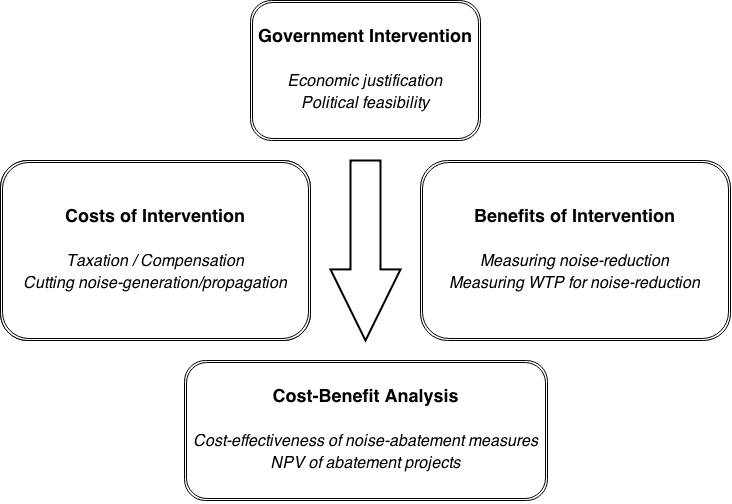
\includegraphics[width=\textwidth]{Graph1}
\end{figure}

\subsection{Justification and feasibility}

Government intervention in the transport sector is ubiquitous due to the public nature of infrastructure and the existence of ``missing markets", such as a market for tranquillity. Noise-abatement policy in road-transport deals with the adverse effects of traffic-noise of third parties. There is a role for economics in the determination of  optimal noise-levels, monetary values of the ``damage done" by noise, and the optimal mix of abatement-measures. 

Next to the economic justification of noise-abatement, policy measures generally need to be politically supported in order for them to be implemented. From this political perspective, providing the public with accurate information can raise support. Furthermore, policy-measures that limit traffic-volume are advised to be accompanied by measures that promote other transport modes.

\subsection{Taxation and compensation}

A first best solution to the problem of traffic noise, is to charge each motorist precisely the amount of external damage caused. Electronic Road Pricing programmes are a real world interpretation of this concept, but deal with political opposition that prohibits implementation. In the special case of aircraft noise, noise-annoyance compensation programmes are considered as a policy measures. Occupants of residences surrounding the airport receive a monetary compensation for the noise-annoyance induced by the airport. In both policy options, there is a need to estimate the external damage of noise. Although the theoretical basis of both types of policy measures is sound, implementing these measures in the road-transport setting might prove a prohibitively large administrative burden.

\subsection{Costs of noise-abatement alternatives}

An economically optimal outcome would require noise to be abated in the most cost-effective manner, up to the point where the marginal abatement-costs equal the marginal benefit of abatement. Estimating the marginal abatement costs requires specific cost information on the different types of noise abatement, and information on the noise-reductions induced by each type of measure. 

\subsection{Measuring physical noise(-reduction)}

\begin{figure}[h]
	\label{Geluidskaart}
	\caption{Part of Geluidskaart 2012 (Sound map 2012) source: Rijkswaterstaat}
	\centering
	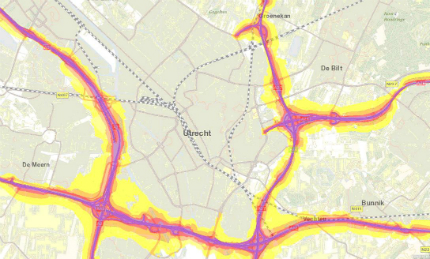
\includegraphics[width=0.8\textwidth]{Geluidskaart}
\end{figure}

The cost-effectiveness of noise-abatement measures can only be evaluated on the basis of the noise-reductions they constitute, in combination with the scope of the measure. For instance, highway noise-barriers amount to great noise-reductions on a very local level, while silent-tires involve a less dramatic noise decrease, but on an national level. Noise-levels are generally measured  in decibel (dB(A)): a logarithmic scale. A doubling of perceived loudness is roughly equal to a 10 dB(A) increase in sound intensity. In the Netherlands, noise-levels surrounding main roads are estimated by Rijkswaterstaat (RWS, road authority), and published in a geographic map format\footnote{ http://www.rijkswaterstaat.nl/geotool/geluidsbelastingrondsnelwegen.aspx}. Figure 3 shows an excerpt of this map, where purple indicates high sound levels(70-75 dB(A)), red 65-69 dB(A), orange 60-64 dB(A) and yellow lower sound levels (55-59 dB(A)). The availability of this type of spatial data indicates that in noise-abatement analysis and evaluation, Geographic Information Systems (GIS) can be of use. Several studies considered in the literature review use GIS in the analysis \citep{Pope2008, Theebe2004}.

\subsection{Measuring willingness-to-pay}

The estimation of WTP for noise-reduction takes up the largest part of economic literature concerning noise-abatement policy.  There are two main roads taken in this strand of literature. One tries to estimate WTP using revealed preference methods, based on real consumer choices. The other estimates WTP by constructing a market for the externality, using stated preference data, based on questionnaires. 

The Hedonic Pricing (HP) method is used to estimate a Noise Depreciation Index (NDI), based on revealed preference data, namely market values of houses. Using this method, one needs to keep in mind the assumptions that lay at the basis of Hedonic Pricing, especially those regarding the workings of the market. \cite{Pope2008} shows that the information environment needs to be properly evaluated, as information asymmetries may bias results towards zero. The use of spatial econometrics, to account for different spatial confounders, is done in many studies, together with Geographic information systems.

Stated preference methods, such as Contingent Valuation (CV) are used to obtain WTP values per person, per year (preferably per dB(A) as well). This value is often translated into a value per household, because data often only shows houses affected by noise (not the amount of occupants)\citep{Nijland2003}. When conduction SP research, one needs to properly account for strategic response behaviour of respondents, and be aware of the hypothetical nature of this type of research. The use of  ``quality of life" survey-techniques, instead of techniques based on monetary values, might deal with some drawbacks of HP (market equilibrium), and SP (strategic response behaviour), but it seems far from bulletproof itself. 

\subsection{Cost-Benefit Analysis}

As it is hard to define general ``units" of noise-abatement, marginal costs and benefits of abatement are often estimated on a project basis, using a Cost-Benefit Analysis (CBA) approach. CBA results in the Net Present Value of all (social) costs and benefits involved in a project. As authorities generally work under budgetary limits, projects might be compared on the basis of their cost effectiveness. The resulting WTP-values from HP and SP analyses may furthermore be used in studies that evaluate the whole array of social costs involved in the transport sector.

\section{Limitations and suggestions}

This paper discusses the current issues in the academic debate concerning noise-abatement analysis. This is done by sketching a research framework that can be used in future studies regarding transport-noise and policy. Although the set of papers evaluated in the analysis is indicative rather than exhaustive, several clear issues emerge from these studies, as discussed in section 4.

Several suggestions for further research can be made, especially with regard to road-transport noise-abatement in the Netherlands. First, to my knowledge there are no recent HP analyses that focus on the effects of road-noise in the Netherlands. Availability of geographical data from the Dutch Highway Authority (RWS) concerning noise levels indicates possibilities for HP Analysis. Second, it seems that in the realm of costs, noise-abatement analysis almost exclusively focuses on source-based costs (silent tires and tarmac) that hamper noise-generation. Costs of measures that hamper noise propagation are largely overlooked, and although the household based WTP values derived from HP methods can readily be applied to housing insulation costs, evaluating the costs and benefits and the optimal supply of noise-barriers requires several more steps. Third, using novel stated preference techniques in combination with road-transport noise-abatement analysis, to deal with methodological issues of HP and CV, deserves further attention. Questions as to the applicability of this method in externality valuation were largely beyond the scope of this literature review, but might be of key interest in further research. 

\bibliography{BibFile}
\bibliographystyle{apalike}
\end{document}
